% -----------------------------------------------------------------------------
% Implementation
% -----------------------------------------------------------------------------
\chapter{Implementation}

As noted before the ANC system has solely been implemented in the simulation environment Matlab. The system consist of several subsystems. These subsystems will be elaborated step by step and their functioning will be demonstrated.\\
The complete source code can be found in the \color{blue}\href{https://github.com/leonardberresheim/MA---Active-Noise-Control-in-Spatial-Domains/tree/main/Matlab}{projects github repository} \color{black} and is free to use, change and share without restrictions.

\section{Spherical Harmonics Decomposition}
The accuracy of the spherical harmonics decomposition in (\ref{eq:primary_noise_field}) with it's truncation degree will be demonstrated using a plane wave \textit{(see figure \ref{fig:planeWaveExp}}) as the exact harmonic coefficients can be calculated using (\ref{eq:plane_wave_coefficients}).
\begin{figure}
    \centerline{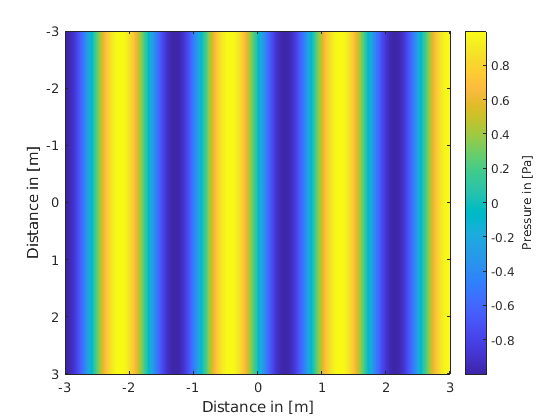
\includegraphics{LaTeX/images/plots/plane_Wave_exponent_form.png}}
    \caption{Plane wave in exponent form}
    \label{fig:planeWaveExp}
\end{figure}

\begin{figure}
    \centerline{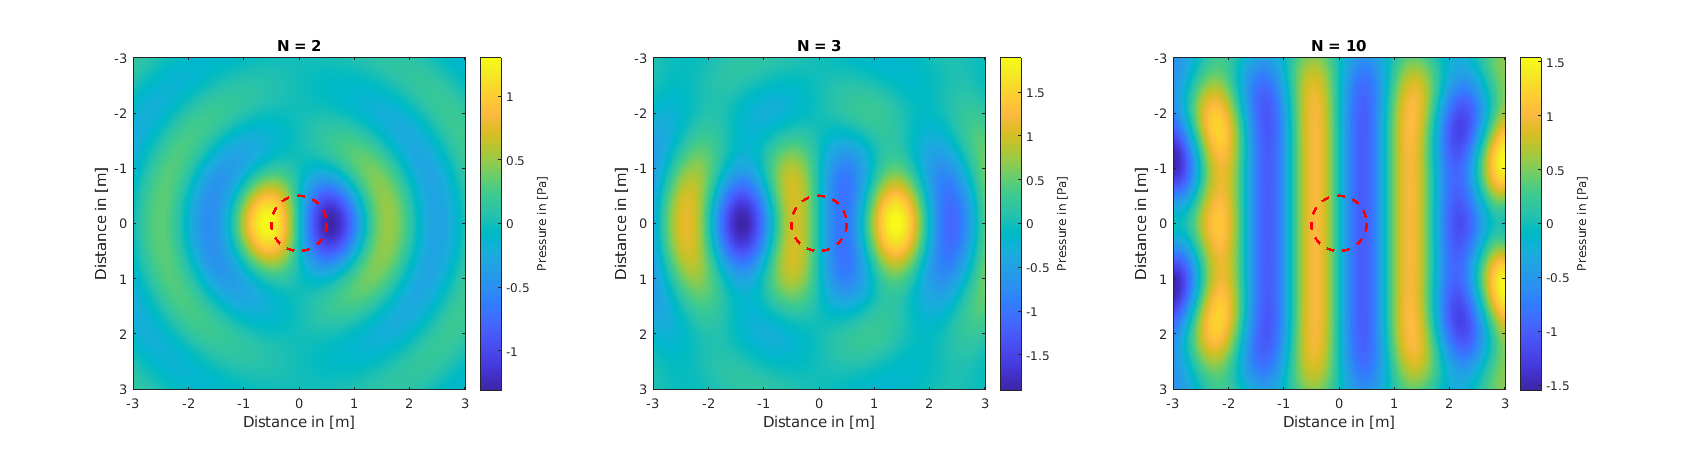
\includegraphics[width=\paperwidth]{LaTeX/images/plots/Plane_wave_harmonics_form.png}}
    \caption{Plane wave in harmonics form for number of modes 2, 3 and 10}
    \label{fig:planeWaveHarmonics}
\end{figure}
When increasing the number of modes the resulting noise field gets closer and closer to the original plane wave in figure \ref{fig:planeWaveExp} as can be seen in figure \ref{fig:planeWaveHarmonics}. However only the quiet zone (\textit{marked as a red circle}) is of interest and with a higher number of modes the number of required loudspeakers increase as well as the computation time. In fact figure \ref{fig:planeWaveHarmonicsError} shows that in the region of interest the accuracy of the spherical harmonics decomposition for $N = 3$ is already adequate.
\begin{figure}
    \centerline{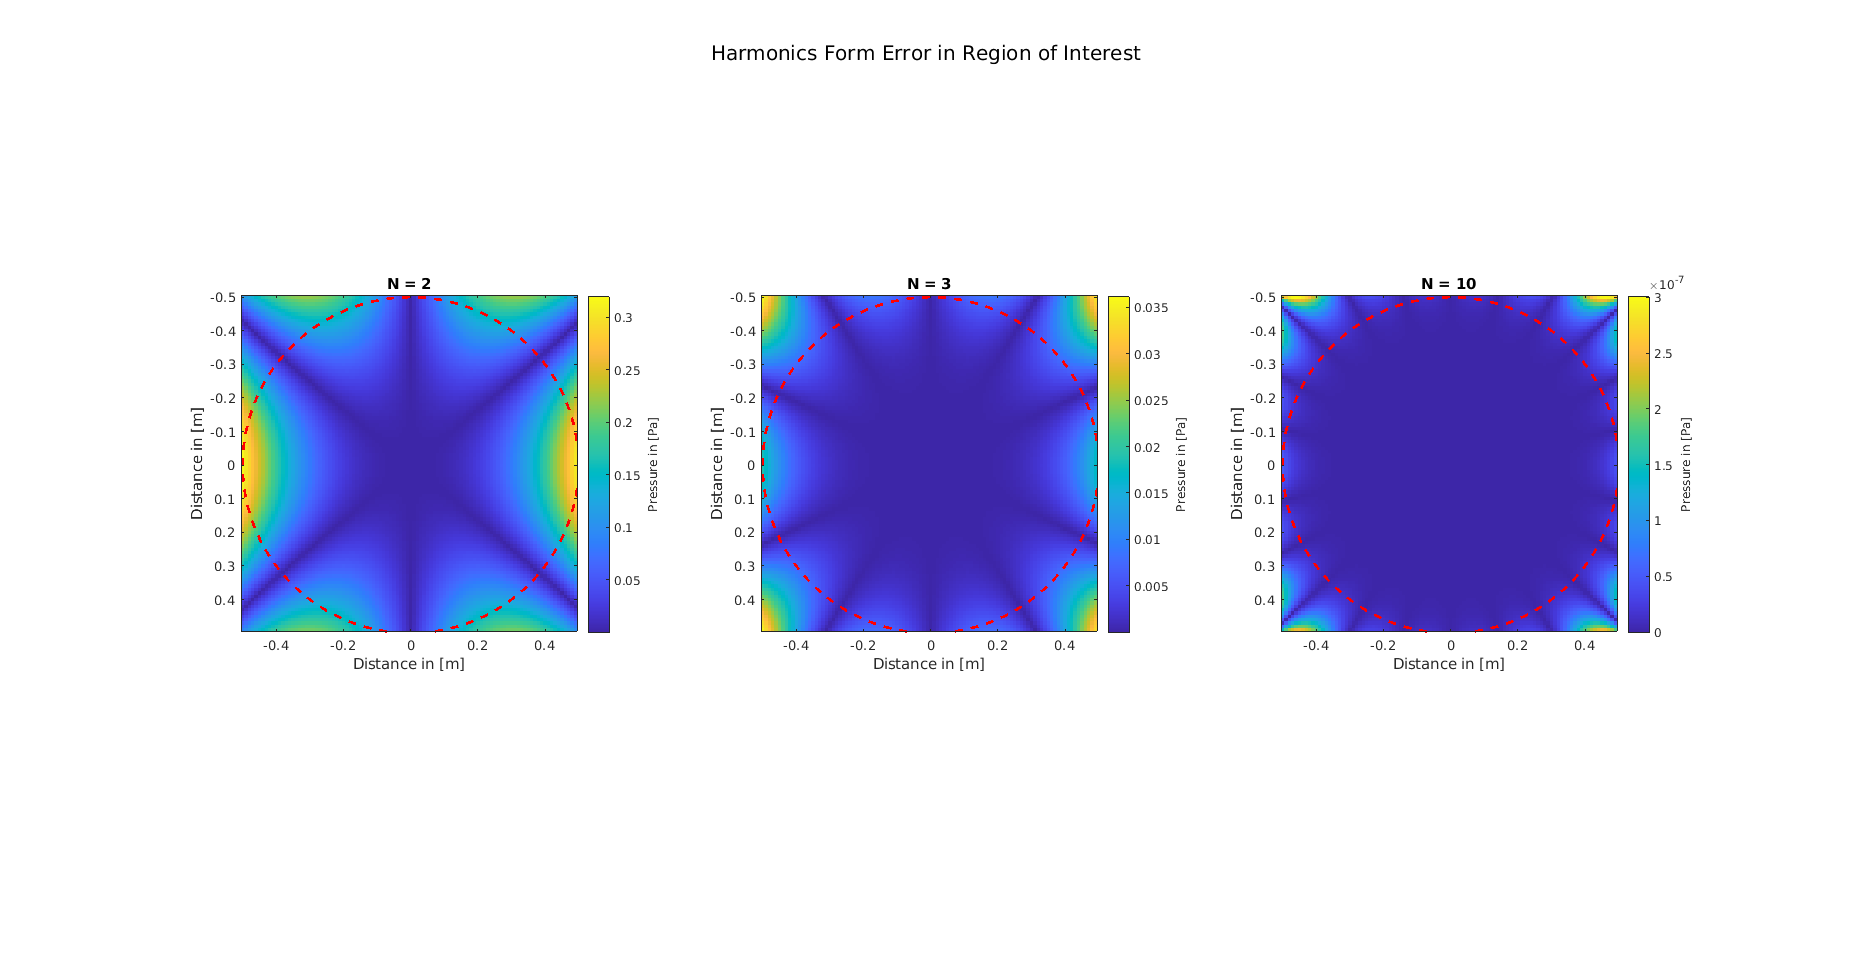
\includegraphics[width=\paperwidth]{LaTeX/images/plots/Plane_wave_harmonics_form_Error.png}}
    \caption{Error of plane wave in harmonics form within region of interest for number of modes 2, 3 and 10}
    \label{fig:planeWaveHarmonicsError}
\end{figure}
\\
\\
\textit{Nota}\\
Only the imaginary part is plotted here as the behavior of the real part of the wave is analogous.
\section{Spherical Microphone Array}
The spherical microphone array is setup around the region of interest according to the Gaussian sampling scheme discussed in \textit{section \ref{sec:Gaussian}} with $2(N+1) = 8$ microphones on the azimuth angle in line with (\ref{eq:azimuth_sample}) and $(N + 1) = 4$ microphones on the elevation angle in line with (\ref{eq:elevation_sample}) resulting in a total of $2(N + 1)^2 = 32$ microphones arranged on the sphere \textit{(see figure }
\begin{figure}
    \centerline{\includegraphics[width=\paperwidth]{LaTeX/images/plots/Microphone_array.png}}
    \caption{Spherical microphone array arranged according to the Gaussian sampling scheme}
    \label{fig:MicrophoneArray}
\end{figure}